\documentclass[xcolor=x11names,compress]{beamer}

%% General document %%%%%%%%%%%%%%%%%%%%%%%%%%%%%%%%%%
\usepackage{graphicx}
\usepackage{tikz}
\usepackage{Tabbing}
\usetikzlibrary{decorations.fractals}
\usepackage{fancyvrb}
%%%%%%%%%%%%%%%%%%%%%%%%%%%%%%%%%%%%%%%%%%%%%%%%%%%%%%

%% Beamer Layout %%%%%%%%%%%%%%%%%%%%%%%%%%%%%%%%%%
\useoutertheme[subsection=false,shadow]{miniframes}
\useinnertheme{default}
\usefonttheme{serif}
\usepackage{palatino}
\usepackage{tabu}
% Links
\usepackage{hyperref}
\definecolor{links}{HTML}{003262}
\hypersetup{colorlinks,linkcolor=,urlcolor=links}

% addition of color
\usepackage{xcolor}
\definecolor{CoolBlack}{rgb}{0.0, 0.18, 0.39}
\definecolor{byellow}{rgb}{0.55037, 0.38821, 0.06142}
\definecolor{dgreen}{rgb}{0.,0.6,0.}
\definecolor{RawSienna}{cmyk}{0,0.72,1,0.45}
\definecolor{forestgreen(web)}{rgb}{0.13, 0.55, 0.13}
\definecolor{cardinal}{rgb}{0.77, 0.12, 0.23}

\setbeamerfont{title like}{shape=\scshape}
\setbeamerfont{frametitle}{shape=\scshape}

\setbeamercolor*{lower separation line head}{bg=CoolBlack}
\setbeamercolor*{normal text}{fg=black,bg=white}
\setbeamercolor*{alerted text}{fg=dgreen} % just testing; I think this looks better
\setbeamercolor*{example text}{fg=black}
\setbeamercolor*{structure}{fg=black}

\setbeamercolor*{palette tertiary}{fg=black,bg=black!10}
\setbeamercolor*{palette quaternary}{fg=black,bg=black!10}

% Margins
\usepackage{changepage}

\mode<presentation>
{
  \definecolor{berkeleyblue}{HTML}{003262}
  \definecolor{berkeleygold}{HTML}{FDB515}
  \usetheme{Boadilla}      % or try Darmstadt, Madrid, Warsaw, Boadilla...
  %\usecolortheme{dove} % or try albatross, beaver, crane, ...
  \setbeamercolor{structure}{fg=berkeleyblue,bg=berkeleygold}
  \setbeamercolor{palette primary}{bg=berkeleyblue,fg=white} % changed this
  \setbeamercolor{palette secondary}{fg=berkeleyblue,bg=berkeleygold} % changed this
  \setbeamercolor{palette tertiary}{bg=berkeleyblue,fg=white} % changed this
  \usefonttheme{structurebold}  % or try serif, structurebold, ...
  \useinnertheme{circles}
  \setbeamertemplate{navigation symbols}{}
  \setbeamertemplate{caption}[numbered]
  \usebackgroundtemplate{}
}


\usepackage{cutwin}

% adding slide numbers
\addtobeamertemplate{navigation symbols}{}{%
    \usebeamerfont{footline}%
    \usebeamercolor[fg]{footline}%
    \hspace{1em}%
    \insertframenumber/\inserttotalframenumber
}

% equation stuff
\usepackage{mathrsfs}
\usepackage[mathcal]{euscript}
\usepackage{amssymb}
\usepackage{amsthm}
\usepackage{epsfig}
\usepackage{amsmath}

% title stuff for footer
\title{Binary Formulation of Decay Equations}
\author{Scopatz, Bates, Wilson}
\date{LANL-XX-XXXX}

% arrow
\usetikzlibrary{shapes.arrows}
\tikzset{
        myarrow/.style={
        draw,
        fill=orange,
        single arrow,
        minimum height=3.5ex,
        single arrow head extend=0.5ex}
}

\newcommand{\arrowdown}{
 \tikz [baseline=-1ex]{\node [myarrow,rotate=-90] {};}
}

%%%%%%%%%%%%%%%%%%%%%%%%%%%%%%%%%%%%%%%%%%%%%%%%%%%%%
\begin{document}



%%%%%%%%%%%%%%%%%%%%%%%%%%%%%%%%%%%%%%%%%%%%%%%%%%%%%%
%%%%%%%%%%%%%%%%%%%%%%%%%%%%%%%%%%%%%%%%%%%%%%%%%%%%%%
\begin{frame}
\title{Binary Formulation of Decay Equations}
%\subtitle{}
\author{\textbf{Cameron~R.~Bates$^{2}$} for Anthony~Scopatz$^{1}$ \\
        \vspace{0.1in}
        Paul Wilson$^{1}$\\
        \vspace{0.1in}
        $^{1}$ The University of Wisconsin-Madison\\
        $^{2}$ Los Alamos National Laboratory}

\date{ANS Summer Meeting, June, 2015}
\titlepage
\end{frame}

%------------------------------------------------------
\begin{frame}{Outline}
    \Large
	\begin{columns}
  	\begin{column}{0.5\textwidth}
	    \begin{itemize}
        \item Motivation
        \item Method Derivation
        \item Results
	    \end{itemize}
  	\end{column}
 	%
 	\begin{column}{0.4\textwidth}
 	   \begin{center}
 	   \begin{figure}
       
\includegraphics[height=4cm]{pyne-icon-big.png}
	   \end{figure}
 	   \end{center}
  	\end{column}
	\end{columns}

\end{frame}

%%%%%%%%%%%%%%%%%%%%%%%%%%%%%%%%%%%%%%%%%%%%%%%%%%%%%%
%%%%%%%%%%%%%%%%%%%%%%%%%%%%%%%%%%%%%%%%%%%%%%%%%%%%%%
\section{Motivation}
\begin{frame}{Motivation}

    There are many situations in which the Bateman equations 
    \cite{bateman1910solution} should be solved for decay channels only, 
    rather than for genric transmutation:
    
    \vspace*{1em}
    \begin{itemize}
        \item Non-reactor components of the nuclear fuel cycle (storage, 
              disposition, transit)
        \item Activation analysis
        \item Dosage calculation
    \end{itemize}

    Many solvers of the Bateman equations are not targeted to this reduced 
    use case.

\end{frame}

%%%%%%%%%%%%%%%%%%%%%%%%%%%%%%%%%%%%%%%%%%%%%%%%%%%%%%
\begin{frame}{Motivation}

    Bateman equations solvers for decay-only calculations can be slow because:
    
    \vspace*{1em}
    \begin{itemize}
        \item They perform a full transmutation calculation but with zero
              neutron flux.
        \item They read in data libraries from disk each calculation.
        \item Perform excess floating-point calculations even for decay
              chanels, which also add algorithimc error.
    \end{itemize}

    For example, ORIGEN v2.2 for decay is O($\approx 1$ sec), most of which is
    I/O.

    \vspace*{1em}
    This does not scale well to large systems, such a fuel cycle with 70k 
    fuel assemblies or reactor dose calculations with 50k volume elements.

\end{frame}

%%%%%%%%%%%%%%%%%%%%%%%%%%%%%%%%%%%%%%%%%%%%%%%%%%%%%%
\section*{}
\begin{frame}[fragile]{Questions?}

    \begin{center}
    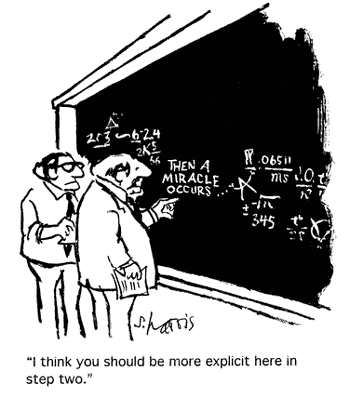
\includegraphics[height=3in,clip]{questions-comic.png}
    \end{center}

\end{frame}

% --------------------------------------------------------------
\begin{frame}[fragile]{PyNE In the Literature}

    \begin{itemize}
    \item Intro: ``PyNE: Python For Nuclear Engineering'' \cite{pyne_intro}
    \item Progress reports: \cite{scopatz_pyne}, \cite{pyne_progress}
    \item In research: \cite{Biondo2014}, \cite{MarquezDamian2014280}, \cite{Scopatz2013a}
    \item V\&V: ``Quality Assurance within the PyNE Open Source \\Toolkit'' \cite{pyne_vnv}
    \item Poster at SciPy: \cite{scipy}
    \end{itemize}

\end{frame}
% --------------------------------------------------------------
\begin{frame}[allowframebreaks]{References}
	\bibliographystyle{unsrt}
    \bibliography{ans.bib}
\end{frame}

\end{document}
